\subsection{Shear heating}\label{sec:simple_shear}
This exercise is performed in an unit square domain composed by $128\times128$ elements. The velocity field is prescribed on the entire domain with
$\bm{v}=(L_y-y)y\bm{e_x}$; viscosity, density and specific heat are fixed to 1, while thermal conductivity and radiogenic energy are fixed to 0. Therefore,
the energy equation (Eq. \ref{eq:energy}) can be simplified as
\begin{eqnarray}
\frac{\partial T}{\partial t}=H_s\nonumber
\end{eqnarray}
and fixing $T(t=0)=0$, the temperature can be find as
\begin{eqnarray}
T(t)=H_s t\nonumber
\end{eqnarray}
In this case we have
\begin{eqnarray}
\dot{\epsilon_{xx}}&=&\frac{\partial u}{\partial x}=0 \nonumber \\
\dot{\epsilon_{yy}}&=&\frac{\partial v}{\partial y}=0 \nonumber \\
\dot{\epsilon_{xy}}&=&\frac{1}{2}\left(\frac{\partial v}{\partial x}+\frac{\partial u}{\partial y}\right)=\frac{1}{2}(L_y-2y)\nonumber
\end{eqnarray}
and, simplifying Eq. \ref{eq:shear}, shear heating can be calculated as
\begin{eqnarray}
H_s(x,y)=(1-2y)^2\nonumber
\end{eqnarray}

The solution predicted by the model in terms of velocity, temperature and shear heating match well with the analytical solutions (Fig. \ref{fig:analytical_en}). 
All data can be found at \url{https://github.com/aleregorda/Benchmarks/tree/main/Energy_equation/Simple_shear}.

%\begin{figure}
%\centering
%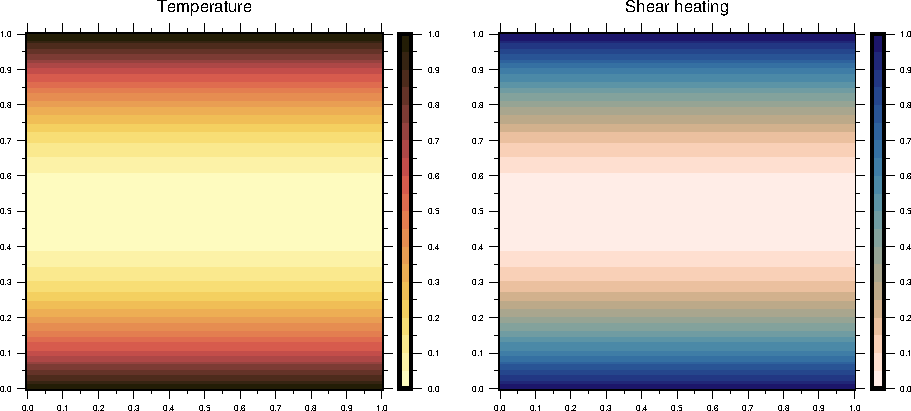
\includegraphics[width=400px]{./Figures/Energy_Thieulot.pdf}
%\caption{Temperature and shear heating predicted by the model after 1 time step.}
%\label{fig:en_thieulot}
%\end{figure}

\begin{figure}[h!]
\centering
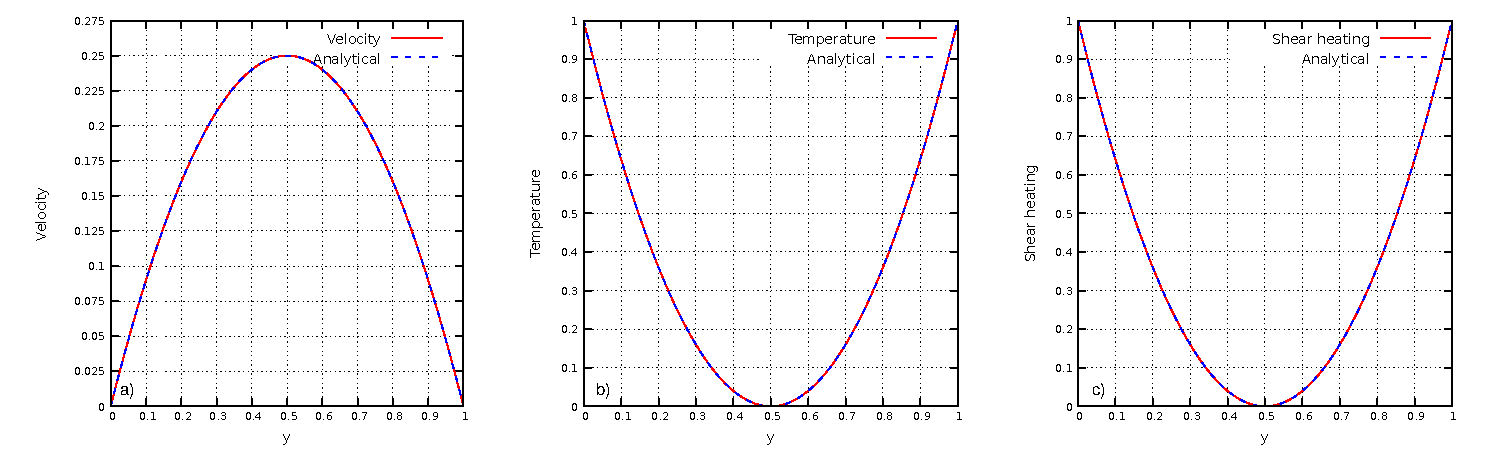
\includegraphics[width=\linewidth]{./Figures/Analytical_Shear.pdf}
\caption{Velocity (panel a), temperature (panel b) and shear heating (panel c) as function of the \textit{y} coordinate for the simple shear experiment. The
solutions predicted by the model (red lines) are compared with the analytical solutions (dashed blue lines).}
\label{fig:analytical_en}
\end{figure}